\section{はじめに}
\subsection{背景}
電離圏研究のための短波ドップラー(HFD)観測データは, オープンデータとして公開され, 自然科学分野で自由に使用できる. \\
現在, データの効率的な再利用を目指し, いくつかのwebアプリケーションが開発されているが, 開発運用やユーザー体験に問題がある. \\
これらのアプリケーションはMySQL, PHP, HTML/CSS, JavaScriptを使用し, 技術の幅広さが開発と保守のコストを増加させている. 
JavaScript(Node.js, React)を用いたアプリケーションも存在するが, データ呼び出しの遅さやインタラクティブ性の不足が課題となっている. \cite{no1}

\subsection{目標}
本研究では既存アプリケーションの問題点から派生した要件について新規開発を行い,  パフォーマンスとUX の向上を実現することを目指す.

\subsection{全体像}
開発の全体像を記す.\\
大きく分けて次の3つのタスクに担当者を分けて開発を行うこととした.
\begin{quote}
	\begin{enumerate}
		\item デザイン作成
		\item バックエンド実装
		\item フロントエンド実装
	\end{enumerate}
\end{quote}

\subsubsection{デザイン作成}
デザイン作成ではクラウドベースのデザインツールであるFigmaを使用して, ワイヤフレームの作成を行いその後に詳細なデザインを構築する. \\
本開発では,ユーザーインターフェース(UI), ユーザーエクスペリエンス(UX), そしてアクセシビリティ(a11y)に配慮した設計の重要性が認識されている. \cite{no2} \\
またコンポーネント単位で統一感のあるデザインが求められるため, デジタル庁が公開しているデザインシステムを参照し極力それに準拠することとした.\cite{no3}\cite{no4}\\
具体的実装は中村が担当する.

\subsubsection{バックエンド実装}
バックエンド実装ではTypeScriptを使用しNext.js上で関数実装を行う. \\
実装内容としては既存サイトからのデータのスクレイピングと整形である. \\
スクレイピングを行う上で, 規約の確認を行った上で実行速度や適切なインターフェースの定義を意識した上で実装を行う必要がある.\\
具体的実装は藤本と中嶋が担当する.

\subsubsection{フロントエンド実装}
フロントエンド実装は大きくUI実装とパフォーマンス・チューニングの2つに分けられる.\\
Next.js上でTailwindCSSを活用したスタイリング実装を行いa11yを意識してUIを実装していく担当と, データ取得部との結合やレンダリングの工夫によりパフォーマンス向上を目指す担当とに分けて実装をおこなう.\\
具体的実装としてはUI実装を中村, 木村, 高橋, データ結合部との結合及びレンダリング実装を中嶋が担当する.

\subsection{本研究の目標}
本研究では, フロントエンド実装のうちデータ取得とページのルーティング・レンダリングに視点を置き, 実行速度や体感的待機時間を意識しての実装と検証について述べるものとする. 

\section{使用技術}
\subsection{Next.jsについて}
Next.jsは, Vercel社が提供するWebフレームワークで, React.jsをベースにしている. \\
その最大の特徴は, 多様なページレンダリング手法のサポートで, 開発者はアプリケーションの特定のニーズに応じて最適なレンダリング戦略を選択できることである.\cite{no5} \\
Next.jsのレンダリングオプションには, クライアントサイドレンダリング(CSR), サーバサイドレンダリング(SSR), スタティックジェネレーション(SG), インクリメンタル静的再生成(ISR)が含まれる. \\
2024年現在, クライアントサイドでのレンダリングをデフォルトとするPage Routerと, サーバーサイドでのレンダリングをデフォルトとするApp Routerの2種類のルーティング手法がある. 本研究ではPage Routerを使用する. 

\subsection{ページレンダリング手法}
\subsubsection{ページレンダリングとは}
Webアプリケーションでのページレンダリングは, ウェブサーバーまたはブラウザがHTML/CSS/JavaScriptなどのコードを解釈し, ユーザーのデバイス上で視覚的なページを表示するプロセスである. 
このプロセスの各ステップの実行タイミングにより分類され, 適切な手法の選定によりサイトの高速化, ユーザー体験の向上, SEOの改善が期待できる. \\
多くのアプリケーションでは, サーバーに送られたリクエストに基づきHTMLを生成・返すServerSideApplicationや, 非同期リクエストを送るAjaxなどが用いられている. \\
近年は, 仮想DOMを用いることでパフォーマンス向上と効率的なUI更新を実現する手法が普及しておりNext.jsでも仮想DOMが使用されている. 
Vercel社のCEO, Guillermo Rauch氏は"7 Principles of Rich Web Applications"の中で, 'Pre rendered pages are not optional'(サーバーによるページの事前レンダリングは必須)と述べている. 
これは, サーバーサイドでのレンダリングがユーザー体験にとって重要であることを示唆している. \cite{no6}\\
本文では, Next.jsで用いられる主要なレンダリング手法とそのメリット・デメリットについて述べる. \cite{no7}

\subsubsection{CSR}
CSR(クライアントサイドレンダリング)は, ウェブページのレンダリングをブラウザで行う手法である. 
サーバーからはHTMLの基本骨格とJavaScriptを送信し, ブラウザがHTMLを動的に生成する. 
この手法は, ウェブページの内容を動的に更新し, ユーザーのインタラクションに応じて即時にコンテンツを変更できるため, SPA(シングルページアプリケーション)の構築に適している. 
また, サーバーへのリクエスト回数が減るため, サーバーの負荷を軽減できるという利点も存在する. \\
しかし, 初回ロード時にJavaScriptのダウンロードと実行が必要で, 表示までの時間が長くなりSEOに不利な点がデメリットである. \\
また, JavaScriptが無効の環境ではコンテンツが正しく表示されないリスクがある. \\
CSRのアーキテクチャ図を図\ref{fig:CSR-image}に示す. 

\begin{figure}[htbp]
	\begin{center}
		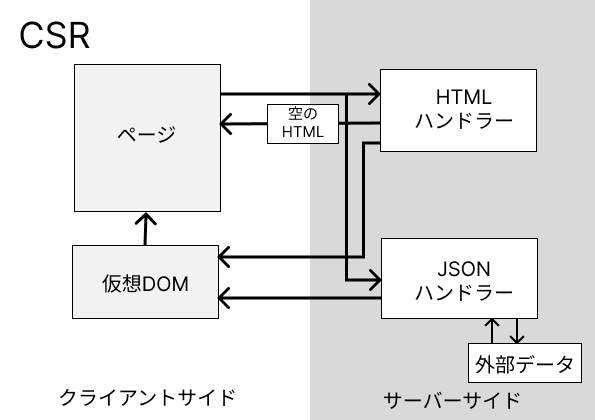
\includegraphics[width=70mm]{./images/CSR.png}
		\caption{CSRのアーキテクチャ}\label{fig:CSR-image}
	\end{center}
\end{figure}

\subsubsection{SSR}
SSR(サーバーサイドレンダリング)は, ウェブページのレンダリングをサーバー側で行う手法である. 
SSRではユーザーのリクエストに応じてサーバーがHTMLを生成し, 完成したページがクライアントに送信される. \\
SSRはクライアントサイドよりも高速なサーバーサイドでHTMLが生成されるため, 初回ページロードの速度が向上しSEOに有効である. 
また, 完成したHTMLが送信されるためSEOに強く, クライアントサイドのJavaScript実行環境に依存しにくい点もメリットである. 
しかし, サーバー負荷が大きい, ページ間移動にリロードが伴う, SGやISRと比べコンテンツの表示に時間がかかるなどのデメリットがある. \\
SSRのアーキテクチャ図を図\ref{fig:SSR-image}に示す. 

\begin{figure}[htbp]
	\begin{center}
		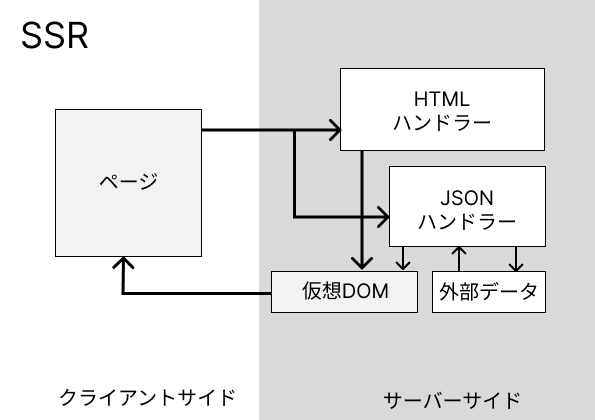
\includegraphics[width=70mm]{./images/SSR.png}
		\caption{SSRのアーキテクチャ}\label{fig:SSR-image}
	\end{center}
\end{figure}

\subsubsection{SG}
SG(スタティックジェネレーション)は, ビルド時に静的なHTMLファイルを生成する手法である. 
SGではビルド時にすべてのページが静的HTMLとして生成され, リクエスト時にはそのHTMLが提供される. \\
このアプローチの大きなメリットは, ビルド時にHTMLが生成されるため, レスポンスが非常に高速であることである. 
しかし, ビルド後の変更が困難で, 動的なページ生成には向かないというデメリットがある. \\
SGのアーキテクチャ図を図\ref{fig:SG-image}に示す. 

\begin{figure}[htbp]
	\begin{center}
		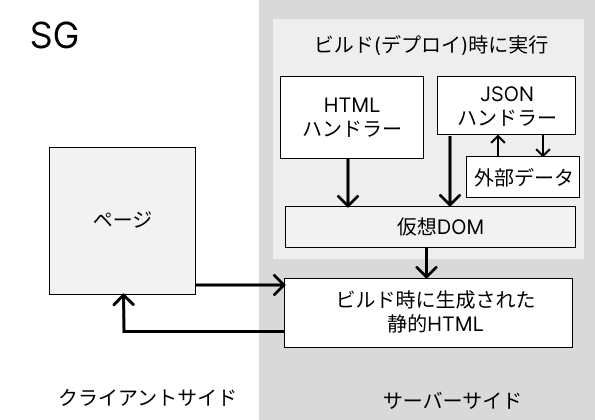
\includegraphics[width=70mm]{./images/SG.png}
		\caption{SGのアーキテクチャ}\label{fig:SG-image}
	\end{center}
\end{figure}

\subsubsection{ISR}
ISR(インクリメンタルスタティックリジェネレーション)は, 静的サイト生成とサーバーサイドレンダリングの組み合わせ手法である. 
ISRではビルド時に一部のページを静的に生成し, 残りのページはユーザーのリクエストに応じて生成・キャッシュされる. 
この方法のメリットは, サイトのビルド時間を短縮しつつ, 動的なコンテンツの提供が可能になる点にありパフォーマンスとコンテンツの更新の柔軟性が両立されている. 
しかし, デメリットとして再生成後の初回リクエスト時にオーバーヘッドが大きく, 読み込み時間が長くなる可能性がある. \\
ISRのアーキテクチャ図を図\ref{fig:ISR-image}に示す. 

\begin{figure}[htbp]
	\begin{center}
		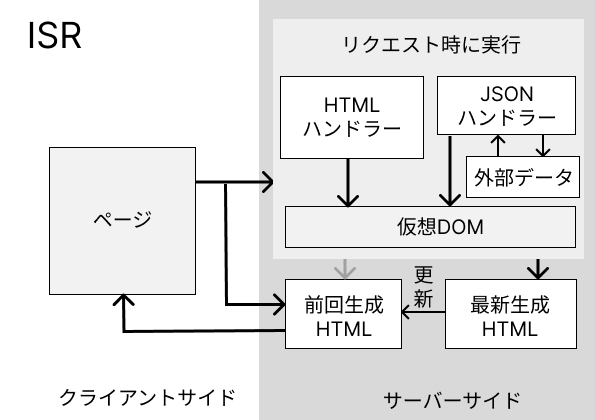
\includegraphics[width=70mm]{./images/ISR.png}
		\caption{ISRのアーキテクチャ}\label{fig:ISR-image}
	\end{center}
\end{figure}

\subsubsection{Next.jsにおけるページレンダリング}
Next.jsにおけるページレンダリングは, ページコンポーネントのライフサイクルとデータ取得方法に依存する. \\
このフレームワークは, 異なるレンダリング手法をページごとに適用する柔軟性を持っている. 
例えば, 単一のアプリケーション内で, 一部のページではSSRを使用して動的にデータを取得し, 他のページではSGを使用して静的に生成することが可能である. \\
この柔軟性により, 開発者はパフォーマンス, SEO, ユーザーエクスペリエンスのバランスを考慮しながら, アプリケーションの特定の要件に合わせて最適なレンダリング戦略を選択できる. 
これにより, 高速で対話的なウェブアプリケーションの構築が可能となり, 結果としてユーザーに優れた体験を提供することが可能となる. 

\subsection{スクレイピングについて}
このアプリケーションでは, 各観測所で観測されたデータを公開している既存アプリケーションからデータをスクレイピングし, 再描画を行う. 
スクレイピングは, webアプリケーションからHTMLデータをクローラで取得し, 必要な情報を抽出する技術のことである. \\
スクレイピング時には, 取得元サイトの規約を遵守する必要がある. 
今回の場合, 取得先のデータがOSS化されており, 学術目的での使用に関して団体から許可を得ているため, 過剰な負荷をかけない範囲での利用が可能と判断した. \\
実装にはSuperagentとCheerioライブラリを用い, Next.js上でTypeScript関数として実装した. \\
一般に, 外部サイトにアクセスする際はCORS(Cross-Origin Resource Sharing)エラーに注意が必要である. 
これは, 異なるオリジン(ドメイン, プロトコル, ポート)からのリソースにクライアントサイドでアクセスしようとした際に生じるセキュリティ問題である.\cite{no8} \\
今回のように異なるドメインのAPIからデータを取得しようとする場合, ブラウザはこれを同一オリジンポリシーによりブロックする可能性がある. 
しかし, 今回はサーバーサイドでのレンダリングを行い, クライアント側で直接アクセスされないため, Next.js上でのスクレイピングにおいてCORSエラーは発生しない. 

\section{アプリケーション設計と実装方法}
\subsection{実装の要件}
本研究では, アプリケーション実装の主要部分として外部データの取得とページの描画に焦点を当てている. 
特に, データフェッチからの画面描画速度の高速化をUX向上のための主要な目標と設定した. 

今回作成するアプリケーションに含まれる, webスクレイピングを伴うページは以下の2つである. 
\begin{quote}
	\begin{itemize}
		\item 波形データの検索ページ\\(index.tsx)
		\item 波形データの描画ページ\\(/data/[type]/[loc]/[year]/[date].tsx)
	\end{itemize}
\end{quote}
これらのページの実装において, ビルド時間とスクレイピングのリクエスト数の2つの軸で最適化を行うこととする. 

\subsection{スクレイピングに用いた関数}
今回実装したスクレイピング関数は二つあり, 一つは指定された日時と観測所の周波数データを取得してCSVからJSONに変換するもの, もう一つは存在するデータの一覧を取得して整形するものである. \\
スクレイピング対象のアプリケーションでは, 観測所, 年度, 日時に従ってネストされたパスから周波数データを取得できる. 
第一の関数では, URLを使って具体的なデータの所在ページを指定し, スクレイピングを行う. 
第二の関数では, 観測所の一つ上の階層から始まり, 子要素のページを再帰的に全探索してスクレイピングし, 整形する. 

\subsection{レンダリング設計}
レンダリング設計に関しては, 以下の二つのパターンで実装し, ビルドにかかる時間を比較して考察する. 
\begin{quote}
	\begin{enumerate}
		\item ISRを用いる方法
		\item SGとSSRを用いる方法
	\end{enumerate}
\end{quote}
これにより, スクレイピングによるデータ取得とページレンダリングの最適な組み合わせを評価する. 

\subsubsection{ISRを用いる方法}
最初の手法は, ISRを用いた実装である. この手法では, ビルド時に一括でスクレイピング処理を行い, 静的なサイトを生成する. \\
実装方法としては, まずgetStaticPaths関数でディレクトリ一覧をスクレイピングし, 静的にビルドされるページを特定する. 
次に, getStaticProps関数を用いて, それぞれのページの波形データを取得しビルドを行う. 
さらに, ISR技術を活用することで, 再ビルドのタイミングを制御し, 定期的に新しく追加されたデータを取得できるように設定する. \\
図\ref{fig:ISR-arc}で, ISRを用いた場合のアプリケーション設計を示す. 

\begin{figure}[htbp]
	\begin{center}
		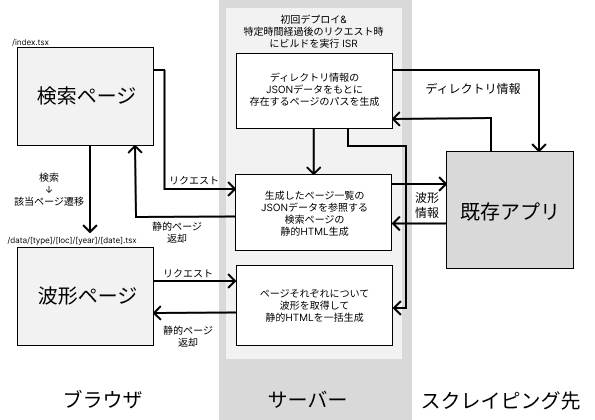
\includegraphics[width=70mm]{./images/app/ISRver.png}
		\caption{ISRを用いた場合の設計}\label{fig:ISR-arc}
	\end{center}
\end{figure}

\subsubsection{SGとSSRを用いる方法}
二つ目の手法は, SGとSSRを組み合わせた方法である. \\
この手法では, ディレクトリの取得と波形データの取得をそれぞれSGとSSRを用いて分離させる. 
具体的な実装方法としては, getStaticPropsを使用して検索ページに存在するパスを静的に生成し, getServerSidePropsを利用して各ページがリクエストされた際に動的に波形データを返すという流れになっている. \\
図\ref{fig:SG-SSR-arc}で, SGとSSRを併用した場合のアプリケーション設計を示す. 

\begin{figure}[htbp]
	\begin{center}
		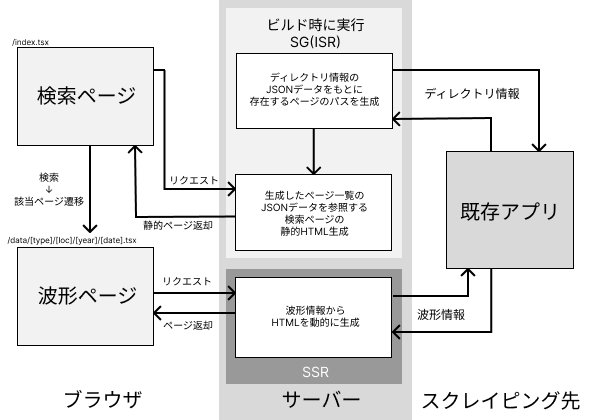
\includegraphics[width=70mm]{./images/app/SG-SSRver.png}
		\caption{SGとSSRを併用した場合の設計}\label{fig:SG-SSR-arc}
	\end{center}
\end{figure}

\subsection{環境}
本研究での実行環境に関して, 使用したPCの仕様を表\ref{table:zikkoukannkyo}に, 使用したパッケージのバージョンを表\ref{table:version}に示す. 

\begin{table}[hbtp]
	\caption{実行環境}
	\label{table:zikkoukannkyo}
	\centering
	\begin{tabular}{lcr}
		\hline
		名称      & MacBookPro    \\
		CPU     & Apple M1 Max  \\
		メモリ     & 32GB          \\
		コマンドシェル & zsh (v1.85.1) \\
		\hline
	\end{tabular}
\end{table}

\begin{table}[hbtp]
	\caption{パッケージのバージョン}
	\label{table:version}
	\centering
	\begin{tabular}{lcr}
		\hline
		名称         & バージョン   \\
		\hline \hline
		Node.js    & 18.12.0 \\
		Next.js    & 13.0.6  \\
		TypeScript & 4.9.4   \\
		\hline
	\end{tabular}
\end{table}


\section{実装結果}
\subsection{データ取得}
本研究での実装において, 2種類の方法いずれでもデータを取得することができた. \\
データ取得の成功は, スクレイピングとレンダリングの設計が適切に機能していることを示している. \\
図\ref{fig:search-page-image}と図\ref{fig:wave-page-image}は, 取得したデータをJSON形式でブラウザ上で表示した様子を示している. 
これにより, データ取得の結果が視覚的に確認できる. 

\begin{figure}[htbp]
	\begin{center}
		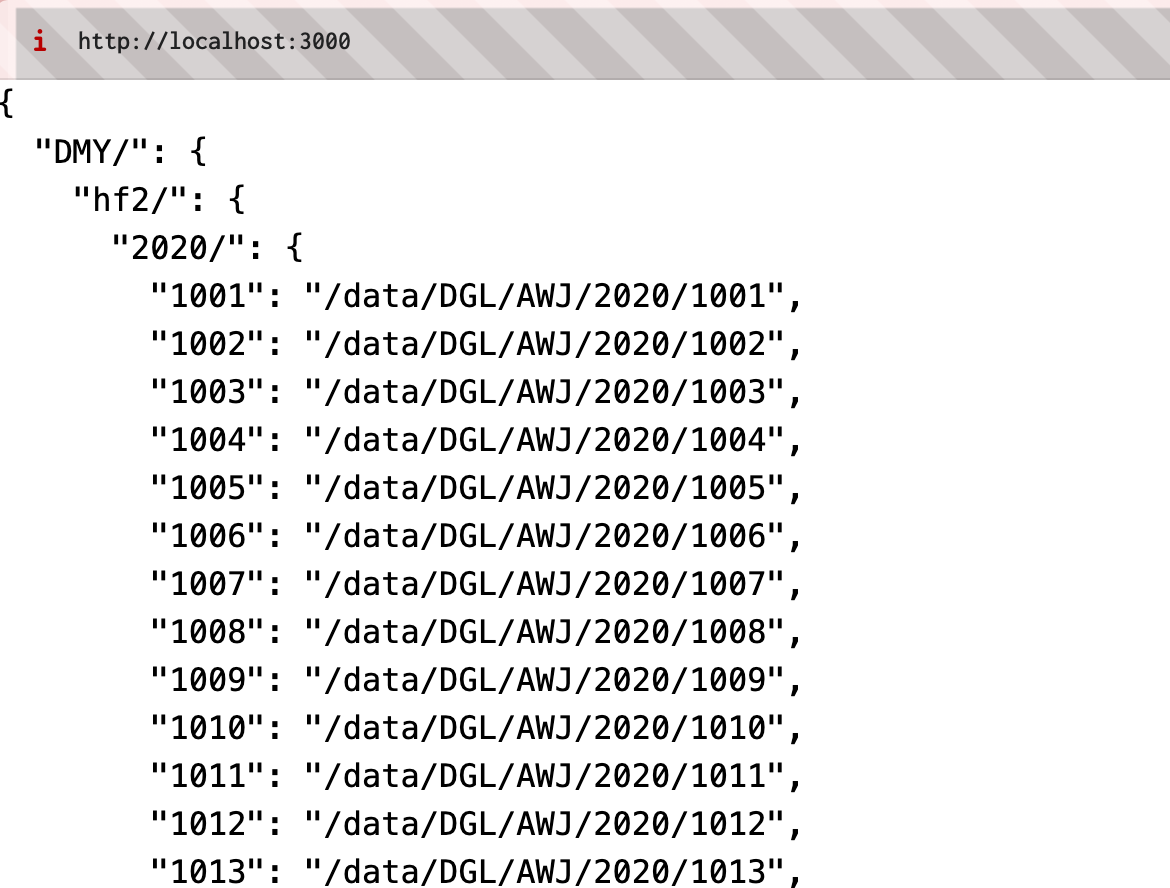
\includegraphics[width=70mm]{./images/search-page-image.png}
		\caption{検索ページでデータ取得している様子}\label{fig:search-page-image}
	\end{center}
\end{figure}

\begin{figure}[htbp]
	\begin{center}
		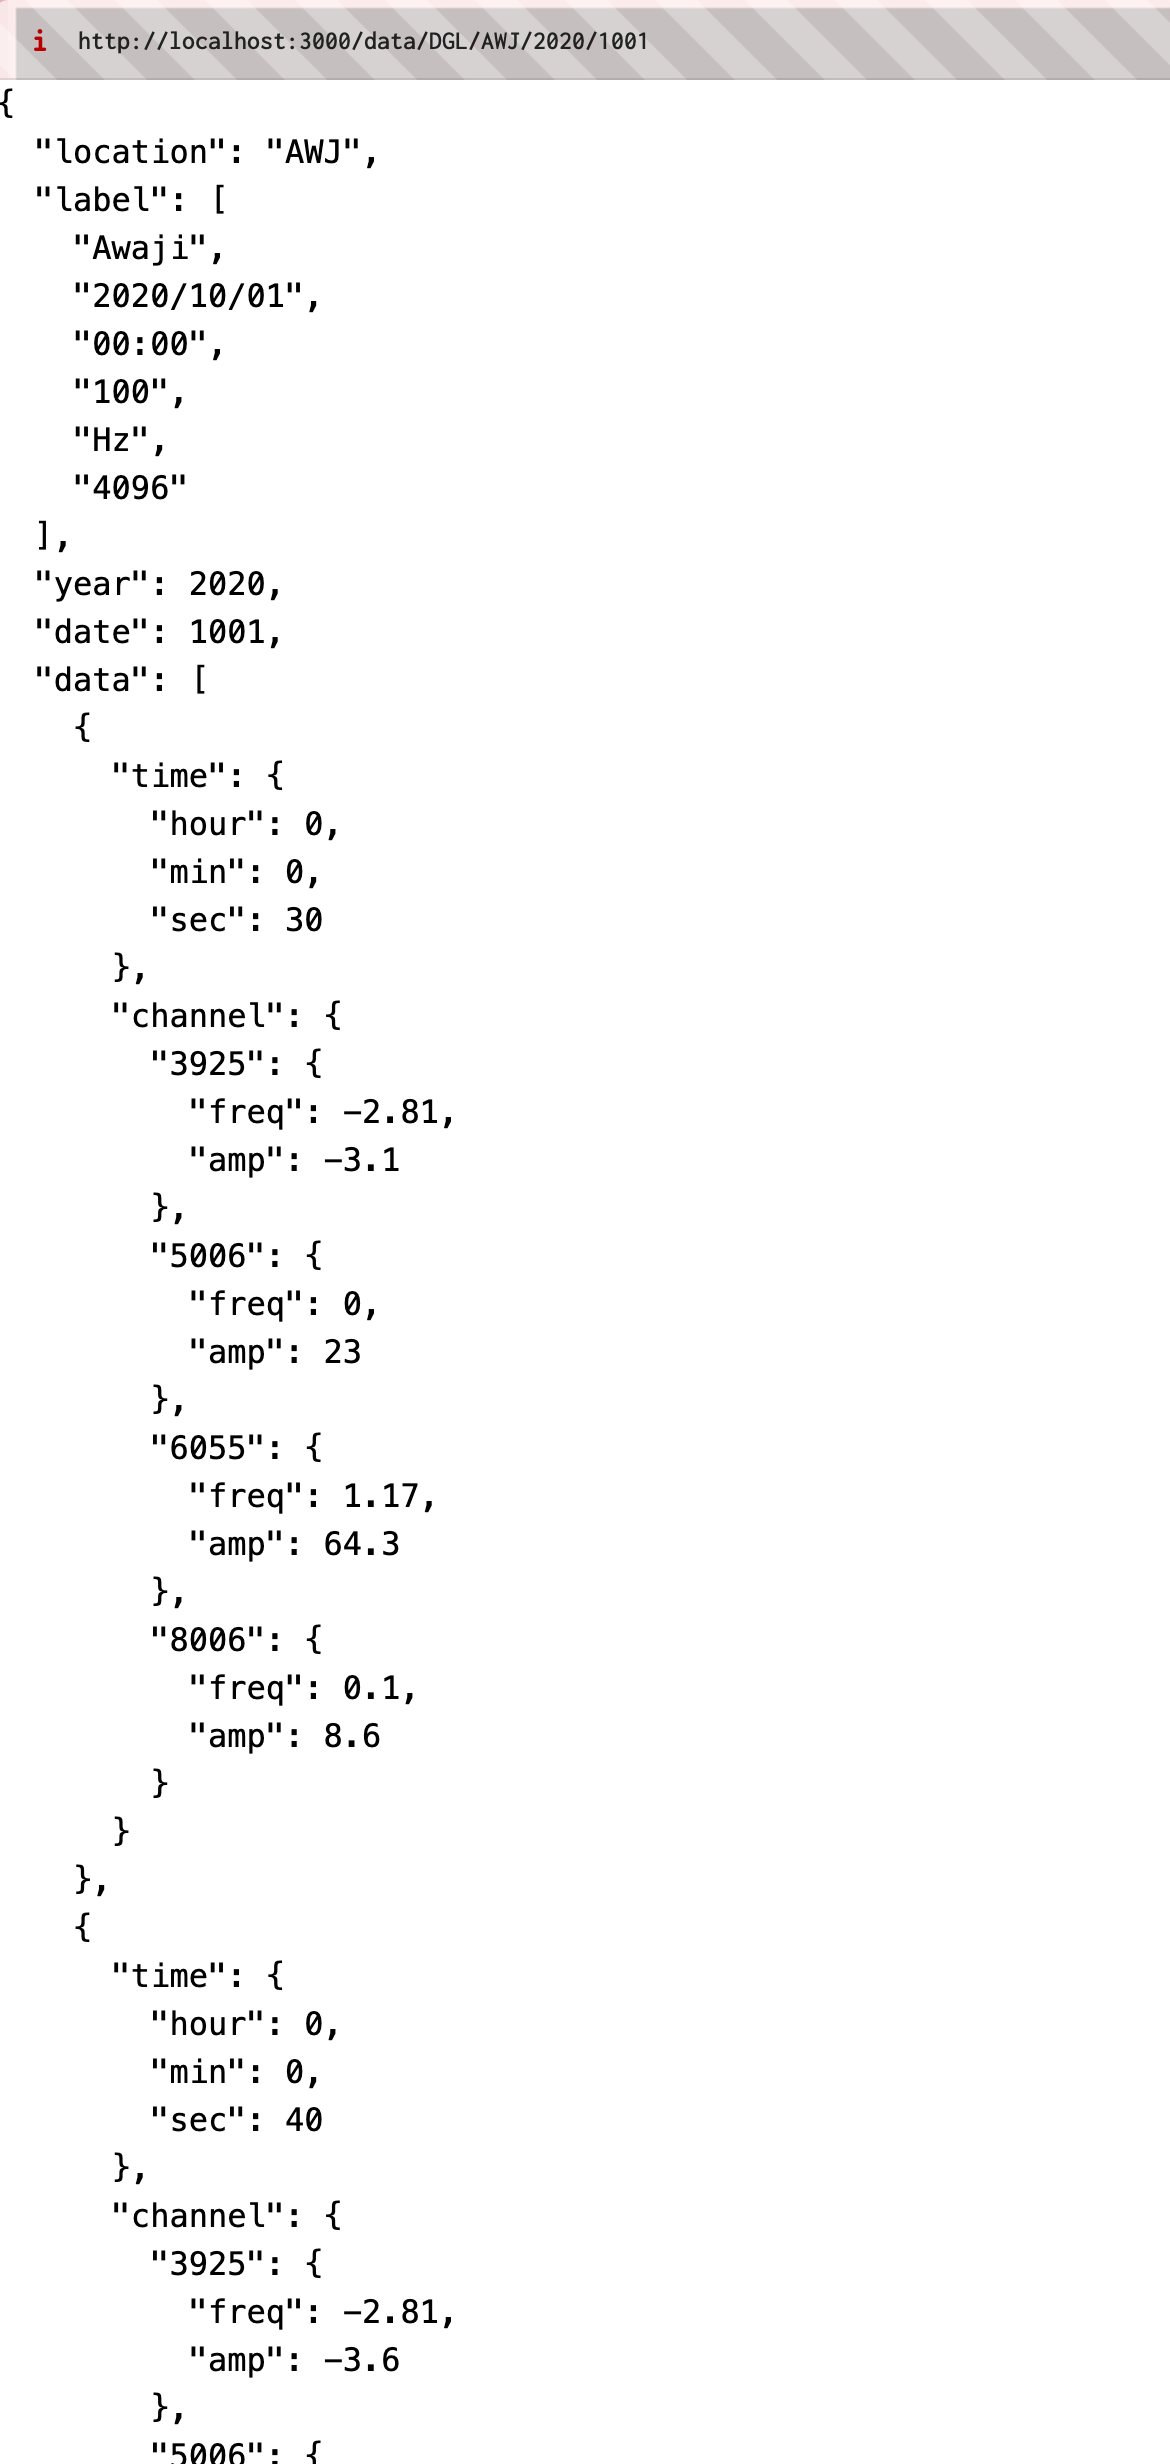
\includegraphics[width=70mm]{./images/wave-page-image.png}
		\caption{波形ページでデータ取得している様子}\label{fig:wave-page-image}
	\end{center}
\end{figure}

\subsection{スクレイピング関数の実行時間}
実装した2つのスクレイピング関数の実行時間について詳述する. \\
実行時間の計測にはperformance.now()メソッドを用い, 関数の実行前後の時間差で測定した. 

\subsubsection{scrapeWaveData}
この関数は, 指定されたデータ形式, 観測所名, 年, 日時を引数として受け取り, 観測データのCSVを取得しJSON形式に変換する. \\
この関数の実行時間を表\ref{table:scrapeWaveData}に示す. 

\begin{table}[hbtp]
	\caption{scrapeWaveDataの実行時間}
	\label{table:scrapeWaveData}
	\centering
	\begin{tabular}{lcr}
		\hline
		回数  & 実行時間(ms) \\
		\hline \hline
		1回目 & 1435     \\
		2回目 & 1166     \\
		3回目 & 1054     \\
		4回目 & 997      \\
		\hline
		平均  & 1163
	\end{tabular}
\end{table}

表\ref{table:scrapeWaveDatay}から, この関数の実行には平均して約1.2秒かかることがわかる. 

\subsubsection{scrapeDirectory}
この関数は, 指定されたURL配下に存在するページを再帰的に全探索し, ディレクトリ名をキーとするネストされたオブジェクトとして返すものである. \\
この関数の実行時間を表\ref{table:scrapeDirectory}に示す. 

\begin{table}[hbtp]
	\caption{scrapeDirectoryの実行時間}
	\label{table:scrapeDirectory}
	\centering
	\begin{tabular}{lcr}
		\hline
		回数  & 実行時間(ms)   \\
		\hline \hline
		1回目 & 319411     \\
		2回目 & 325276     \\
		3回目 & 263359     \\
		4回目 & 261885     \\
		\hline
		平均  & 292482.75
	\end{tabular}
\end{table}

表\ref{table:scrapeDirectory}から, この関数の実行には平均して約292秒かかることがわかる. 

\subsection{静的ビルドの実行時間の比較}
ISRを用いる手法とSGとSSRを併用する方法との2パターンでビルドを実行し, ビルドログに出た実行時間を示す.
\subsubsection{ISRを用いる方法}
ISR(SG)を用いて, ビルド時に存在するパスを生成した後各ページまでを静的に生成する方法を用いた場合のビルドログを図\ref{fig:ISR-build}に示す.

\begin{figure}[htbp]
	\begin{center}
		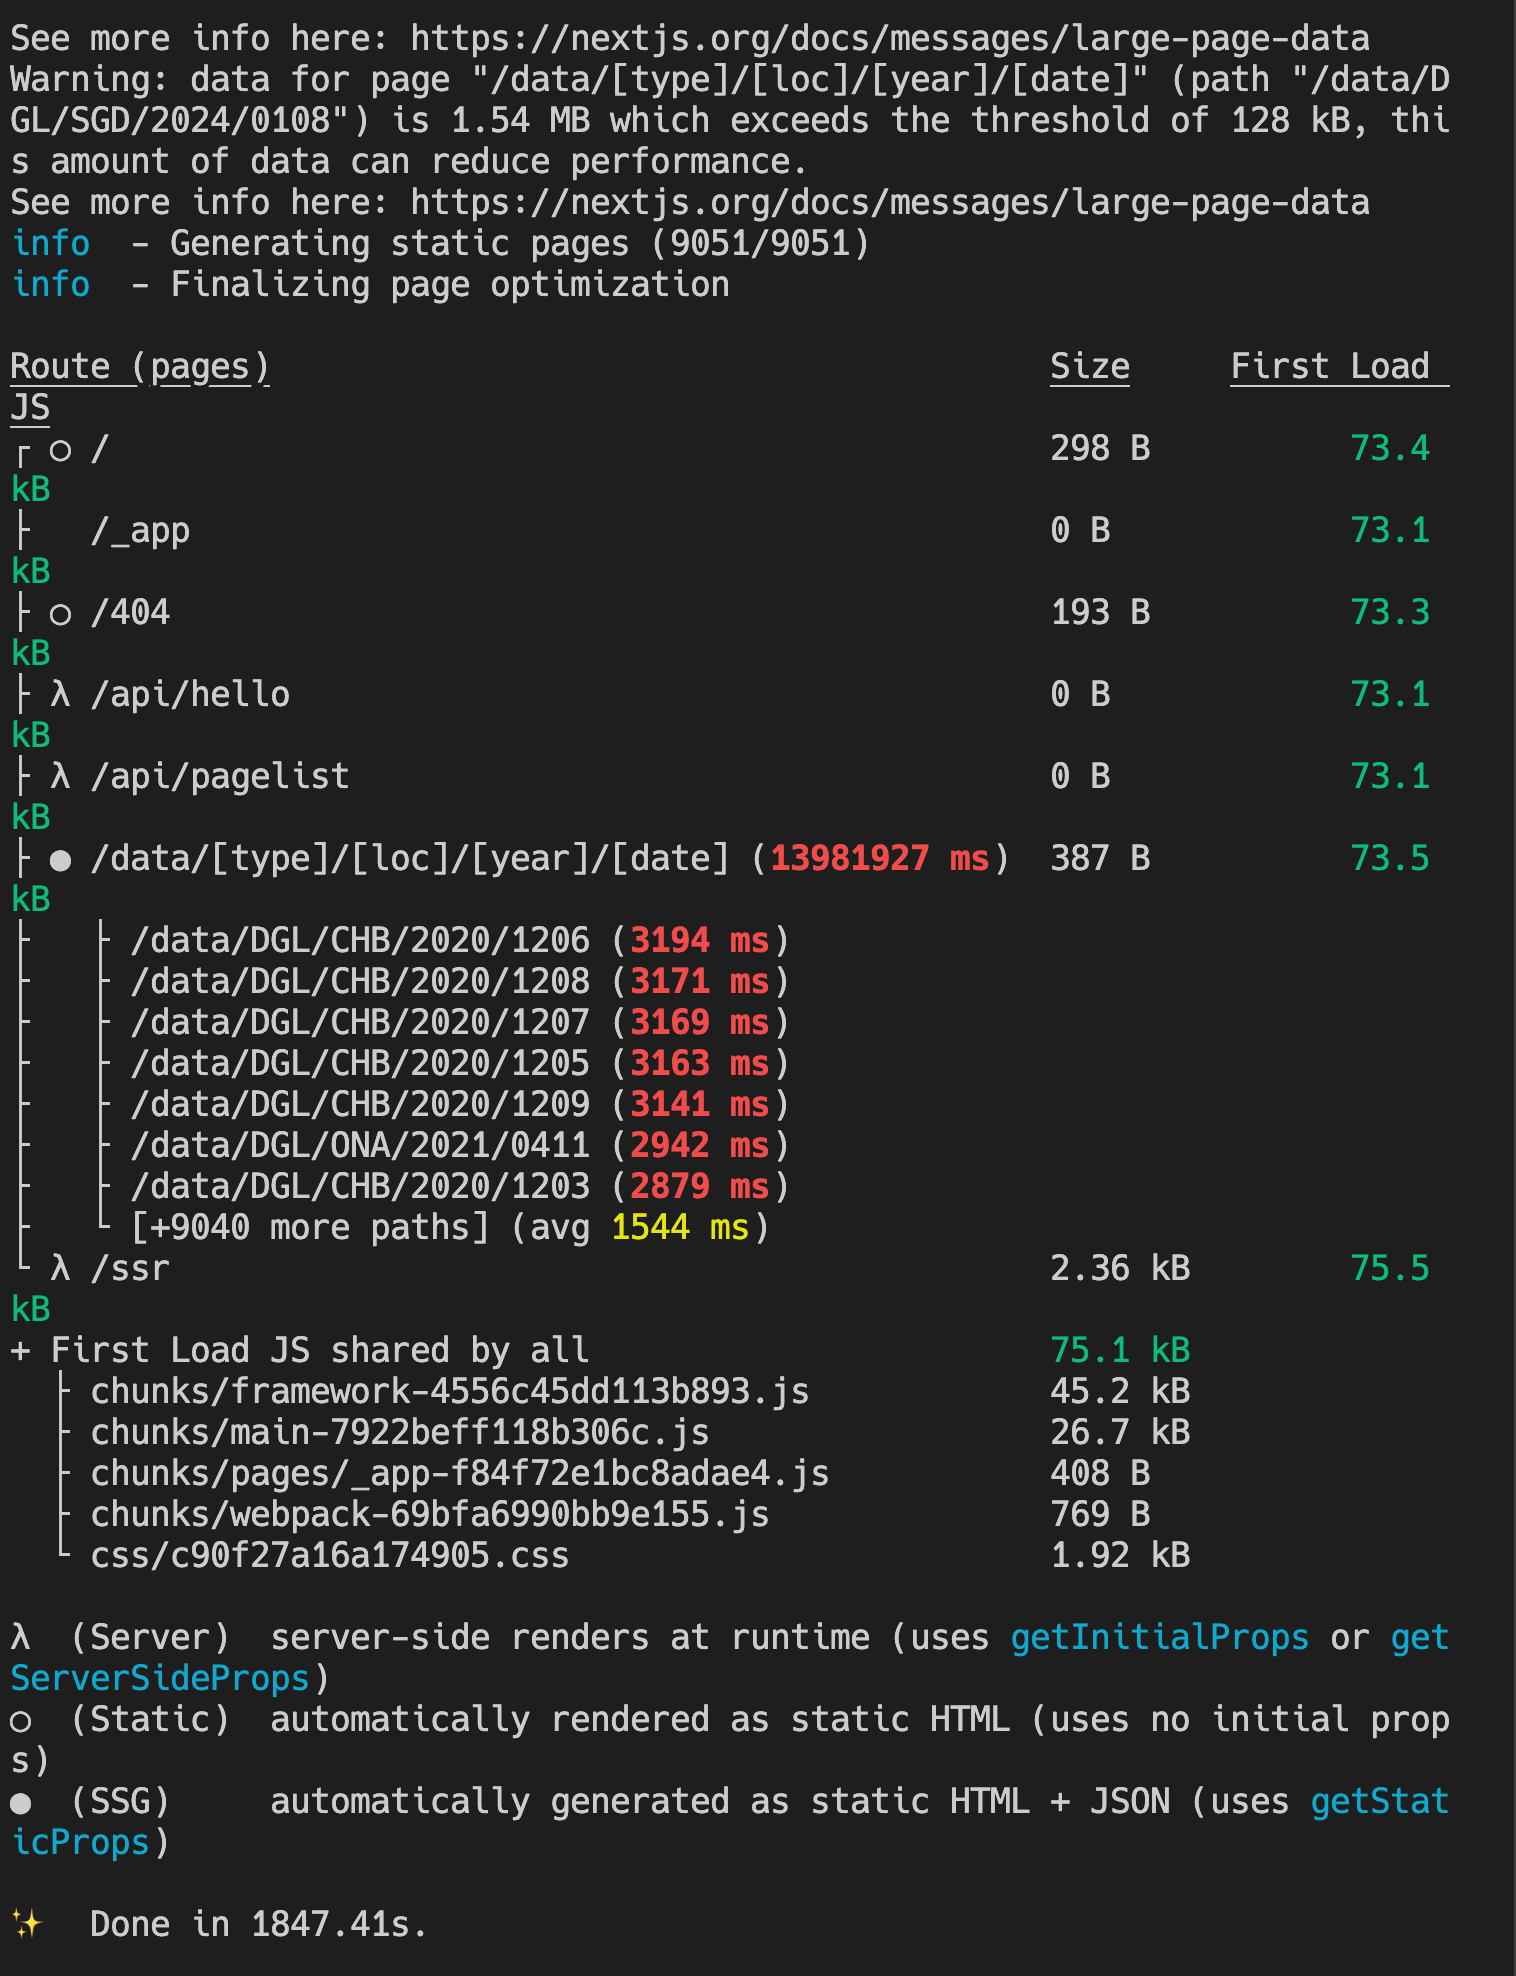
\includegraphics[width=70mm]{./images/ISR-log.png}
		\caption{ISR(SG)を用いた際のビルドログ}\label{fig:ISR-build}
	\end{center}
\end{figure}

実行結果からビルド時間は約188秒であることが確認できる.

\subsubsection{SGとSSRを用いる方法}
SGとSSRを併用して, ビルド時には存在するパスのみを静的に生成しておき各ページはアクセスされた際に動的に生成した場合のビルドログを図\ref{fig:SG-SSR-build}に示す.

\begin{figure}[htbp]
	\begin{center}
		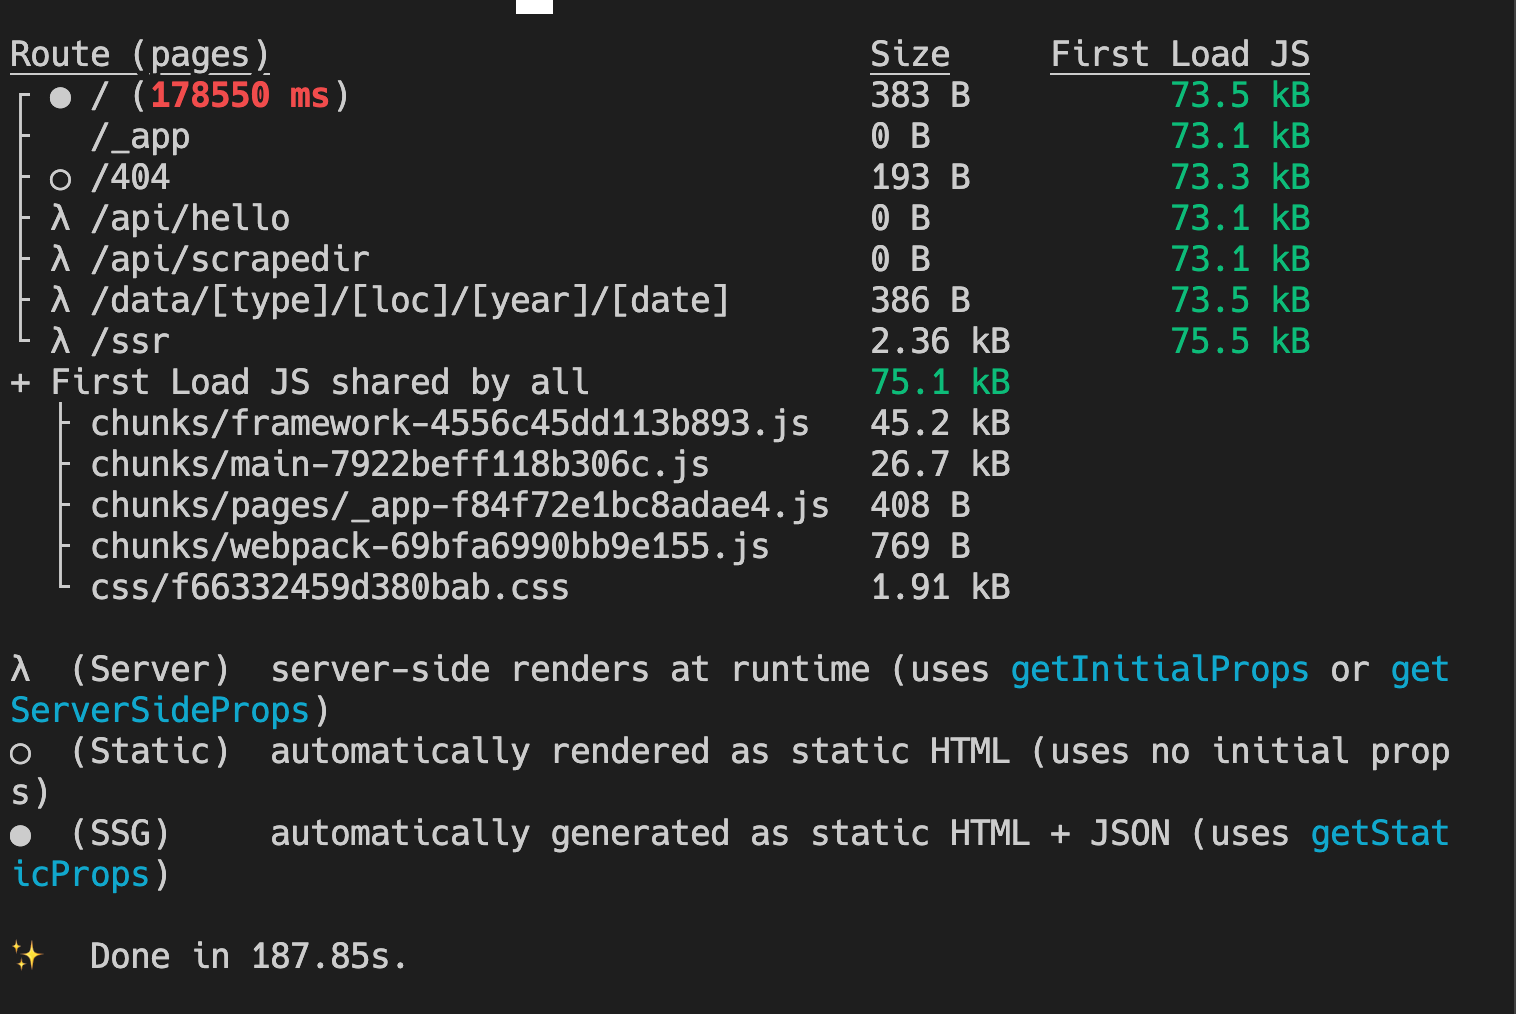
\includegraphics[width=70mm]{./images/SGandSSR-log.png}
		\caption{SGとSSRを併用した場合のビルドログ}\label{fig:SG-SSR-build}
	\end{center}
\end{figure}

実行結果からビルド時間は約1847秒であることが確認できる.

\section{考察}
\subsection{スクレイピングの実行結果について}
スクレイピングの実行結果から, ディレクトリ情報の取得には波形データの取得よりも多くの時間が必要であることが明らかになった. 
これは, 波形データの取得が一度のページアクセスで済むのに対し, ディレクトリ情報の取得にはディレクトリ全体を探索する必要があり, その結果, 複数回のページアクセスが必要になるためである. \\
この結果は, スクレイピングの効率化に向けた改善の必要性を示唆している. 

\subsection{ビルドの実行結果について}
ビルド時間の比較結果によれば, ISRを用いた場合のビルド時間は, SGとSSRを併用した場合の約10倍であることが確認できる. 
この結果は, ISRを用いる場合には, スクレイピング処理と静的ファイル生成のための時間が著しく増加することを示している. 
この差は, 特に大規模なサイトや頻繁に更新されるコンテンツを扱う際に, ビルドの効率性を考慮する上で重要な考慮点となる. 

\subsection{ビルド方法の選定}
本研究での実装結果を踏まえ, アプリケーションのビルド方法の選定について考察する. \\
ISRの使用ではビルド時間に約30分かかることが確認された. 
ISRの定期再ビルド機能を考慮すると, 初回アクセス時のビルド時間が実質的なオーバーヘッドとなり, ユーザーが長時間待たされる可能性がある. 
これはユーザーエクスペリエンスの観点から見て適切ではない. \\
一方, SGとSSRを併用した場合, ページへの移行時に約1秒のスクレイピング時間が発生する. 
ISRと比較して多少の時間はかかるが, オーバーヘッドの問題を考慮すると, これは許容範囲内であると考えられる. 
SGの欠点として, 動的なページ生成が難しい点があるが, 本アプリケーションではスクレイピング元のサイトでデータの追加が1日に数回であるため, GitHub ActionsなどのCI/CDツールを用いて定期的な再ビルドを行うことで対応が可能である. \\
ISR単体またはSG単体の使用と比較して, CI/CDツールを用いた再ビルドの方が, GitHub Actionsの料金体系を考慮しても, 長いビルド時間によるコスト増加を抑えることができる. \\
したがって, これらの理由から本研究ではSGとSSRを併用することが現状において最適な手法と結論づけた. 
この方法では, ユーザー体験, ビルドの効率性, コストのバランスを適切に取ることができる. 


\subsection{結果を踏まえた追加仮説}
本実験の結果から, SGとSSRを併用する方法が適切であるとの結論に至ったが, この方法ではデータページへのアクセス時にSSRで行われるデータフェッチに約1秒かかることがUX上の課題となる. \\
この課題に対し, プリフェッチ技術の活用によりさらなる高速化が可能であるという新たな仮説を立てた. 
プリフェッチとは, 次にアクセスする可能性が高いページのデータを事前に取得しておく技術である. \\
Next.jsにはNextLink機能があり, 現在表示されているページ上の遷移リンクに関する情報をプリフェッチすることができる. \\
主要なユースケースとして, 以下のフローが考えられる.

\begin{enumerate}
	\item データの検索ページにアクセスする.
	\item データを検索し, リンクから任意のデータページにアクセスする.
\end{enumerate}

この仮説では, データ検索ページで任意のデータページへの遷移リンクを表示した際にプリフェッチを行うことで, 実際にアクセスされた際のデータ取得よりも高速化が期待できる. \\
しかし, Next.jsのドキュメントと有志の技術ブログによると, SSR時に使用されるgetServerSidePropsにおいてはNextLinkによるプリフェッチが実行されない. 
この場合, クライアントサイドでのデータ取得を行い, 次ページのプリフェッチを行う方がユーザー体験の速度向上に寄与する可能性がある.\cite{no9} \\
さらに, useSWRというReact Hooksライブラリを使用することで, キャッシュ戦略とプリフェッチを最適化することも考えられる.\cite{no10} \\
これらの仮説に対しては, 実際に実装して検証する必要があり, その価値は十分にあると考えられる. 
このような最適化は, ユーザー体験の向上に大きく寄与し, アプリケーションの全体的なパフォーマンスを高める可能性を秘めている. 


\section{おわりに}
本研究では, 電離圏研究のための短波ドップラー観測データをスクレイピングし, 再描画するアプリケーションにおけるレンダリング戦略について調査と検証を行った. \\
研究結果を踏まえ, 適切なUI実装を施すことにより, 高速でユーザーエクスペリエンス(UX)的に優れたアプリケーションの作成が可能であると確信している. 
さらに, 考察時に提出した追加仮説に関しても, 調査を行い, それらを導入することで, UXの向上という観点からさらに有益な実装が可能になると考えられる. \\
この研究は, データを効率的にスクレイピングし, ユーザーフレンドリーなインターフェースで提示するアプローチを示しており, 今後の電離圏研究をサポートするアプリケーション開発において重要な指針となるだろう. \\
現時点での実装成果としてアプリケーションの完成までには至らなかったが, 本研究で得られた知見・実装は目的の一つであったUX向上に対しアプリケーションの高速化という点で一定の成果となったのではないかと考える.\\
今後の実装としては分担して行った実装を統合する必要がある. 実装完了後にユーザーからのフィードバックを得ることによって, より実際のユースケースに即したUX向上につなげることができるだろう.

\begin{thebibliography}{99}
	\bibitem{no1}
	仲純平, 短波ドップラーデータ公開用Webアプリケーションの開発, 特別研究公開発表会, 北九州工業高等専門学校, 2022
	\bibitem{no2}
	ソシオメディア株式会社 上野学 藤井幸多, オブジェクト指向UIデザイン 使いやすいソフトウェアの原理, 技術評論社, 東京, 2020
	\bibitem{no3}
	デジタル庁, デザインシステム | デジタル庁, https://www.digital.go.jp/policies/servicedesign/designsystem/
	\bibitem{no4}
	伊原力也 小林大輔 桝田草一 山本怜, Webアプリケーションアクセシビリティ 今日から始める現場からの改善, 技術評論社, 東京, 2023
	\bibitem{no5}
	Vercel, Next.js by Vercel - The React Framework, https://nextjs.org, (参照2024-1-20)
	\bibitem{no6}
	Guillermo Rauch, 7 Principles of Rich Web Applications, https://rauchg.com/2014/7-principles-of-rich-web-applications, (参照2024-1-20)
	\bibitem{no7}
	手島拓也 吉田健人 高林佳稀, TypeScriptとReact/Next.jsでつくる実践Webアプリケーション開発, 技術評論社, 東京, 2022
	\bibitem{no8}
	オリジン間リソース共有(CORS), https://developer.mozilla.org/ja/docs/Web/HTTP/CORS (参照2024-1-20)
	\bibitem{no9}
	Next.jsのprefetchに関して, https://taroodr.com/posts/nextjs-prefetch (参照2024-1-20)
	\bibitem{no10}
	Vercel, SWR, https://swr.vercel.app/ja, (参照2024-1-20)
\end{thebibliography}